\documentclass{tietreport}

\usepackage{graphicx}
\usepackage{array}
\usepackage{booktabs}
\usepackage{enumitem}
\usepackage{float}
\usepackage{needspace}
\usepackage{xurl} % Allow long URLs in references to break cleanly across lines
\usepackage{tikz}
\usetikzlibrary{arrows.meta,positioning,fit,shapes.geometric}

\usepackage[
  date=year,
  style=alphabetic,
  backend=biber,
  sorting=nyt,
  maxnames=5,
  minnames=3,
  maxalphanames=4,
  minalphanames=3,
  backref=true,
  doi=false,
  isbn=false,
  url=true,
  eprint=false
]{biblatex}
\addbibresource{references.bib}

% Replace the clearly marked administrative placeholders with the submitted details.
\TitlePageHeader{SOFTWARE ENGINEERING (UCS503)}
\ProjectTitle{AI Twin}
\ProjectSubTitle{A Personal Digital Replica for Memory, Behavioural Modelling, Decision Simulation, and Adaptive Goal Support}
\author{%
  \texttt{102403078} Lakkshya Jha \\
  \texttt{1024030713} Saksham Raj \\
  \texttt{1024030697} Noorsharn Singh%
}
\TitlePageSubText{Group: \texttt{3C52} \\ BE Third Year, Computer Engineering}
\AdvisorName{PARAMVEER KAUR}
\TitlePageFooterText{{%
    \large Mid-Semester Evaluation \\[0.2cm]
    \bfseries Computer Science and Engineering Department%
  } \\[0.15cm]
  Thapar Institute of Engineering and Technology, Patiala%
}

\begin{document}
\let\cleardoublepage\clearpage
\maketitle
\pagenumbering{roman}
\tableofcontents
\clearpage
\pagenumbering{arabic}

\chapter{Introduction}

\Needspace{8\baselineskip}
\section{Background and Context}
Artificial intelligence assistants are commonly designed to respond to the immediate prompt presented by a user. Although such systems can provide useful explanations and recommendations, an interaction-by-interaction approach may not consistently represent a person's long-term preferences, experiences, habits, commitments, or goals. A user may therefore need to repeat relevant context, and generic recommendations may not reflect the constraints of that individual's everyday life.

AI Twin proposes a more personalised approach: a digital representation of an individual that can be updated as information is accumulated over time. The project's central idea is to connect personal memory with a dynamic user model, behavioural pattern analysis, decision simulation, and goal-oriented adaptation. Rather than treating every interaction independently, the proposed system aims to use relevant historical context to explain its predictions and tailor its recommendations.

The project is currently in development. Its present stage is requirements and architecture, and the next milestone is the design and implementation of the Personal Memory System. Accordingly, this report documents the proposed system, its design rationale, development plan, and evaluation approach. It does not claim that the complete system or the proposed capabilities have already been implemented or experimentally validated.

\Needspace{8\baselineskip}
\section{Project Status}
The project repository is available at \url{https://github.com/lakkshyajhaaa/UCS503P_202627_Alter}. AI Twin is currently at the requirements-and-architecture stage, with the design and implementation of the Personal Memory System identified as the next milestone. Specific implementation details and test outcomes are not asserted unless supported by project evidence.

\clearpage
\Needspace{8\baselineskip}
\section{Problem Statement}
A conventional assistant may provide advice without maintaining a structured, evolving representation of the user's experiences and behaviour. This creates several related challenges: personal context may be lost between sessions; recommendations may not account for the user's actual schedule and habits; predictions may lack an explicit explanation of the evidence used; and the system may not learn systematically from whether earlier recommendations were followed or successful.

The problem addressed by AI Twin is the design of a privacy-conscious personal system that can organise user-controlled memories, infer patterns from available history, simulate likely decisions in a given context, and adapt goal-related recommendations based on feedback. These outputs must distinguish stored facts from inferred preferences and predictions, and they must remain open to user correction.

\Needspace{8\baselineskip}
\section{Aim and Objectives}
The overall aim is to design a modular personal AI system that follows the cycle \textit{Remember, Understand, Predict, Adapt, and Learn}. The objectives are:
\begin{enumerate}[leftmargin=*]
  \item \textbf{Design persistent personal memory:} specify semantic, episodic, and behavioural memory categories and the operations required to create, retrieve, update, correct, and delete memories.
  \item \textbf{Define a dynamic user model:} represent preferences, goals, knowledge, behaviours, and patterns, with updates driven by new interactions and observed outcomes.
  \item \textbf{Specify evidence-aware decision simulation:} design a process that estimates a likely user choice from relevant context and communicates confidence and supporting factors without presenting a prediction as a fact.
  \item \textbf{Plan adaptive goal support:} represent goals, schedules, commitments, priorities, distractions, and past adherence so that future plans can be personalised.
  \item \textbf{Establish an evaluation framework:} define measures for memory retrieval, preference and decision prediction, recommendation usefulness, and behavioural adaptation before reporting empirical performance.
  \item \textbf{Address privacy and user control:} incorporate consent, data minimisation, secure storage, transparency, and memory management into the proposed design.
\end{enumerate}

\clearpage
\Needspace{8\baselineskip}
\section{Scope and Limitations}
The initial scope is a single-user AI Twin. The proposed system is intended to support personal memory, user modelling, decision simulation, adaptive goal optimisation, behavioural pattern detection, and learning from outcomes. The planned technical direction includes a modular AI layer, local or open-weight models where permitted, embeddings and retrieval, a Python/FastAPI backend, a React or Next.js frontend, and PostgreSQL with pgvector or an alternative vector store.

These technologies are options in the project plan, not a verified record of the final implementation. The initial report therefore focuses on requirements and design. Multimodal inputs, long-term temporal analysis, environmental intelligence, and broader simulation are treated as future possibilities rather than completed features.

\chapter{Methodology and Design}

\Needspace{8\baselineskip}
\section{Development Methodology}
The project follows a phased development roadmap. The phases provide a staged method in which foundational requirements and memory capabilities precede behavioural modelling and higher-level decision support.
\begin{enumerate}[leftmargin=*]
  \item \textbf{Research and requirements:} define scope, study related approaches, specify memory and behavioural requirements, identify evaluation metrics, and finalise the architecture.
  \item \textbf{Memory system:} develop a user profile, data ingestion, semantic and episodic memory, persistent storage, retrieval, and memory management.
  \item \textbf{User modelling:} extract preferences, process behavioural data, detect patterns, update the profile, and maintain confidence indicators.
  \item \textbf{Twin engine:} combine contextual retrieval with personalised response generation, decision simulation, and evidence-based predictions.
  \item \textbf{Adaptive goal optimisation:} represent goals and schedules, detect constraints, analyse habits, optimise plans, and track interventions.
  \item \textbf{Evaluation and integration:} create an evaluation dataset, test retrieval and prediction, analyse failure cases, refine the interface, improve performance, and document security and deployment considerations.
\end{enumerate}

\Needspace{8\baselineskip}
\section{System Architecture}
The architecture is modular so that individual components can be developed, tested, and replaced independently. The user interacts through a client interface. An interaction API passes input to processing and goal-management components. Relevant information is stored in the memory system and retrieved for the user model, behavioural analytics, and knowledge representation. The Twin Engine uses the retrieved context to reason, predict, and optimise; an adaptation layer presents personalised output and collects feedback for subsequent updates.

\begin{figure}[htbp]
\centering
\resizebox{0.96\textwidth}{!}{%
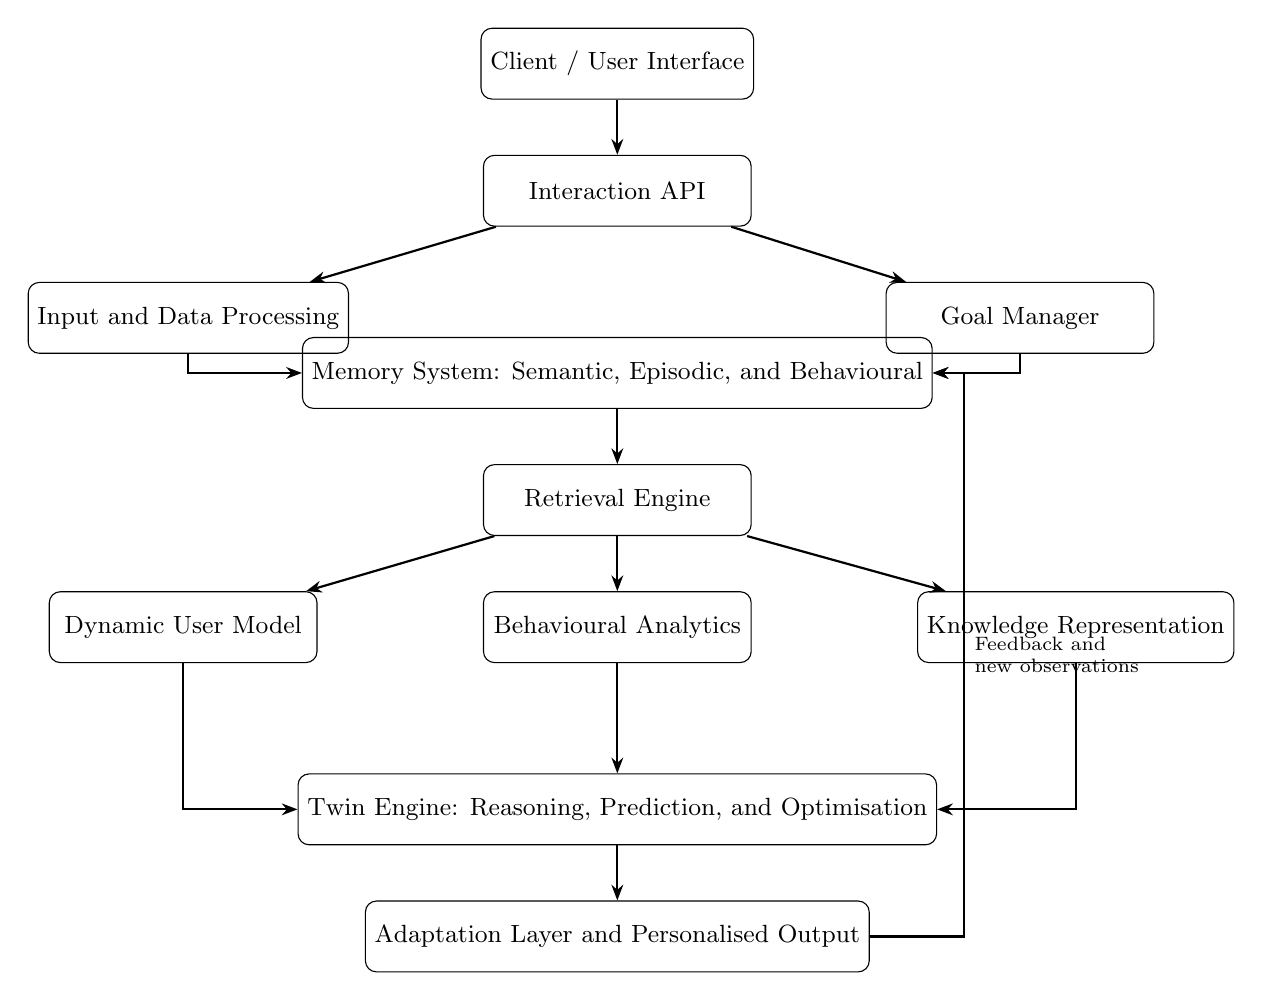
\begin{tikzpicture}[
  node distance=7mm and 13mm,
  block/.style={draw, rounded corners, align=center, minimum width=34mm, minimum height=9mm, font=\small},
  wide/.style={draw, rounded corners, align=center, minimum width=50mm, minimum height=9mm, font=\small},
  flow/.style={-{Stealth[length=2mm]}, thick}
]
\node[block] (ui) {Client / User Interface};
\node[block, below=of ui] (api) {Interaction API};
\node[block, below left=of api, xshift=-4mm] (input) {Input and Data Processing};
\node[block, below right=of api, xshift=4mm] (goal) {Goal Manager};
\node[wide, below=14mm of api] (memory) {Memory System: Semantic, Episodic, and Behavioural};
\node[block, below=of memory] (retrieval) {Retrieval Engine};
\node[block, below left=of retrieval, xshift=-8mm] (user) {Dynamic User Model};
\node[block, below=of retrieval] (analytics) {Behavioural Analytics};
\node[block, below right=of retrieval, xshift=8mm] (knowledge) {Knowledge Representation};
\node[wide, below=14mm of analytics] (twin) {Twin Engine: Reasoning, Prediction, and Optimisation};
\node[wide, below=of twin] (adapt) {Adaptation Layer and Personalised Output};
\draw[flow] (ui) -- (api);
\draw[flow] (api) -- (input);
\draw[flow] (api) -- (goal);
\draw[flow] (input) |- (memory);
\draw[flow] (goal) |- (memory);
\draw[flow] (memory) -- (retrieval);
\draw[flow] (retrieval) -- (user);
\draw[flow] (retrieval) -- (analytics);
\draw[flow] (retrieval) -- (knowledge);
\draw[flow] (user) |- (twin);
\draw[flow] (analytics) -- (twin);
\draw[flow] (knowledge) |- (twin);
\draw[flow] (twin) -- (adapt);
\draw[flow] (adapt.east) -- ++(12mm,0) |- node[pos=0.25,right,font=\scriptsize,align=left] {Feedback and\\new observations} (memory.east);
\end{tikzpicture}%
}
\caption{Proposed high-level architecture of AI Twin.}
\label{fig:architecture}
\end{figure}

\subsection{Major Components}
\begin{description}[leftmargin=!,labelwidth=35mm,style=nextline]
  \item[Client and interaction API] Accept user goals, questions, corrections, and feedback, then route requests to the relevant subsystem.
  \item[Input processing] Organise incoming information and attach useful metadata such as source, time, and context. The final extraction method remains an implementation decision.
  \item[Goal manager] Maintain user-defined goals, priorities, schedules, and constraints for goal-oriented planning.
  \item[Memory system] Separate stable personal information from event-based history and behaviour-related observations.
  \item[Retrieval engine] Retrieve potentially relevant memories using semantic similarity, metadata filters, and ranking. Retrieved items should retain enough provenance to support explanation and correction. Semantic embeddings can support meaning-based retrieval, as explored in Sentence-BERT~\cite{reimers2019}, while retrieval-augmented approaches provide a general design precedent for combining retrieved context with generated outputs~\cite{lewis2020}.
  \item[User model and behavioural analytics] Maintain an evolving representation of preferences and goals and analyse recurring activity patterns when sufficient data is available.
  \item[Twin Engine] Use relevant memories and model features to produce personalised reasoning, likely-choice estimates, and goal-plan suggestions.
  \item[Adaptation layer] Present outputs, collect feedback, and record outcomes for later evaluation and model updates.
\end{description}

\Needspace{14\baselineskip}
\section{Personal Memory Design}
The proposed design uses three complementary memory categories. Their separation is important because a stable preference, a specific past event, and a pattern inferred from repeated actions have different meanings and confidence requirements.
\begin{table}[htbp]
\centering
\small
\begin{tabular}{p{28mm}p{53mm}p{55mm}}
\toprule
\textbf{Memory type} & \textbf{Purpose} & \textbf{Illustrative contents from the project concept} \\
\midrule
Semantic & Store relatively stable facts about the user. & Skills, interests, preferences, goals, knowledge, and important facts. \\
Episodic & Record events and experiences. & Projects, previous conversations, experiences, events, and past decisions. \\
Behavioural & Represent repeated actions and observed tendencies. & Productive periods, recurring choices, distractions, routine deviations, and decision patterns. \\
\bottomrule
\end{tabular}
\caption{Proposed personal memory categories.}
\label{tab:memory}
\end{table}

Each memory should ideally include its content, category, source, creation or observation time, and status. Additional confidence or provenance metadata may help distinguish direct user statements from system inferences. These fields are design recommendations for the proposed system and must be finalised during implementation. Memory management should support viewing, correcting, updating, and deleting stored information, as a core requirement of the proposed design.

\Needspace{8\baselineskip}
\clearpage
\section{Dynamic User Model and Decision Simulation}
The user model is intended to evolve as new interactions and observed behaviours become available. Preferences, goals, and knowledge inform the interpretation of behavioural observations; repeated observations may contribute to patterns, which can in turn inform a decision estimate. Updates should not silently convert uncertain inferences into confirmed facts.

For a hypothetical decision, the planned workflow is:
\begin{enumerate}[leftmargin=*]
  \item Receive a scenario and identify the choice or outcome to be estimated.
  \item Retrieve memories and observations relevant to the scenario, current priorities, and similar past decisions.
  \item Evaluate the available evidence and identify factors that support or contradict candidate choices.
  \item Produce a predicted choice with a confidence estimate and an explanation of relevant factors.
  \item Keep the prediction separate from a normative recommendation; a likely choice is not necessarily the best choice.
  \item When the actual choice becomes known, record the outcome where the user has consented and use it for evaluation and potential model updates.
\end{enumerate}

Confidence must be calibrated through evaluation rather than treated as inherently reliable. If there is insufficient relevant history, the system should communicate uncertainty instead of presenting an unsupported prediction.

\Needspace{8\baselineskip}
\section{Adaptive Goal Optimisation}
The goal-management component is intended to help users pursue goals such as examination preparation, skill development, exercise, project completion, or consistent writing. Personalised ranking and recommendation are established areas of study; the project should select and evaluate a suitable method rather than assume that a particular algorithm is best~\cite{ricci2015}. Planning should consider existing schedules, commitments, habits, productive periods, distractions, historical adherence, preferences, and goal priorities.

The planned adaptation loop consists of defining a goal, collecting constraints, proposing a plan, observing whether tasks were followed, assessing outcomes, and adjusting later plans. Behavioural examples are illustrative only; they are not measured results from this project. The effectiveness of the approach will need to be tested using actual user-approved observations and predefined metrics.

\clearpage
\section{Proposed Technical Stack}
The project has not finalised its technology stack. The following table lists the options currently under consideration.
\begin{table}[H]
\centering
\small
\begin{tabular}{p{35mm}p{100mm}}
\toprule
\textbf{Layer} & \textbf{Technologies or approaches under consideration} \\
\midrule
Backend & Python and FastAPI \\
Frontend & React or Next.js \\
Data storage & PostgreSQL; pgvector or another vector database; optional graph database \\
AI and machine learning & Local or open-weight models where permitted, sentence embeddings, NLP, classification, clustering, recommendation algorithms, behavioural prediction, and time-series analysis \\
Libraries & PyTorch, scikit-learn, spaCy, and Sentence Transformers \\
Retrieval and knowledge & Vector search, semantic retrieval, metadata filtering, memory ranking, and knowledge graphs \\
Engineering and infrastructure & Git/GitHub, Docker, automated testing, and CI/CD \\
\bottomrule
\end{tabular}
\caption{Technical options under consideration; final selections are pending confirmation.}
\label{tab:stack}
\end{table}

The project explicitly aims not to depend on a direct hosted LLM API. The exact local model, embedding model, database configuration, deployment environment, and interface framework remain to be selected and validated. The architecture should therefore keep the AI layer replaceable so that candidate models and algorithms can be evaluated independently.

\Needspace{12\baselineskip}
\clearpage
\section{Privacy, Security, and Ethics}
The system is intended to process highly personal information. The project design identifies user-controlled memory, editing and deletion, transparent evidence for predictions, clear separation of facts and inferences, secure storage, minimal data collection, and explicit consent for behavioural tracking as design goals.

The implementation should apply these principles throughout the data lifecycle. A structured privacy-risk approach can help translate privacy principles into design and governance activities~\cite{nistprivacy2020}. Access to stored information should be restricted; sensitive information should not be collected unless necessary for a clearly explained purpose; retention and deletion behaviour should be documented; and users should be able to inspect or correct information attributed to them. The interface should distinguish at least three states: a known statement, an inference based on observations, and a prediction about a future event. These are requirements to implement and evaluate, not claims that the controls are already operational.

\chapter{Results and Evaluation}

\Needspace{8\baselineskip}
\section{Current Project Status}
The project is marked as \textit{In Development}, with the current stage listed as \textit{Requirements \& Architecture}. The next milestone is the design and implementation of the Personal Memory System. Based on that stated status, this report records the architecture and proposed evaluation plan; it does not report a completed prototype, measured model accuracy, user-study findings, or deployment results.

\Needspace{8\baselineskip}
\section{Testing Methodology}
Testing will be introduced as the corresponding modules are implemented. The following strategy is proposed for the development roadmap.
\begin{itemize}[leftmargin=*]
  \item \textbf{Unit testing:} test memory creation, categorisation, updating, deletion, metadata handling, retrieval ranking, and goal-constraint processing as separate components.
  \item \textbf{Integration testing:} verify the flow from user input through storage and retrieval to the Twin Engine and personalised output, including feedback updates.
  \item \textbf{Functional testing:} check that users can view, correct, update, and delete memories, and that outputs distinguish predictions from recommendations.
  \item \textbf{Privacy and security testing:} verify consent paths, access restrictions, deletion behaviour, and the handling of information that should not be retained.
  \item \textbf{User evaluation:} once a working prototype exists, ask consenting participants to assess relevance, clarity, perceived usefulness, trust, and ease of correction. The evaluation procedure and participant count must be documented before testing.
\end{itemize}

\clearpage
\Needspace{8\baselineskip}
\section{Evaluation Metrics}
The project design identifies several evaluation dimensions. The exact dataset, baseline, thresholds, and experimental protocol remain to be specified before measurements can be reported.
\begin{table}[htbp]
\centering
\small
\begin{tabular}{p{35mm}p{52mm}p{49mm}}
\toprule
\textbf{Dimension} & \textbf{Candidate measures} & \textbf{Evaluation approach} \\
\midrule
Memory retrieval & Precision, recall, and Top-$K$ retrieval accuracy & Compare retrieved memories with a manually labelled set of relevant memories. \\
Preference prediction & Prediction accuracy and consistency & Compare predicted preferences with known or explicitly confirmed user preferences. \\
Decision simulation & Accuracy, confidence calibration, and prediction consistency & Evaluate scenarios for which the user's actual decision is known. \\
Behavioural adaptation & Task adherence and outcome change & Compare predefined measures before and after an intervention, using a documented observation period. \\
User feedback & Personalisation, relevance, accuracy, usefulness, trust, and consistency & Collect structured ratings and qualitative feedback from consenting users. \\
\bottomrule
\end{tabular}
\caption{Proposed evaluation framework. No measured scores are available in the current project description.}
\label{tab:metrics}
\end{table}

\Needspace{8\baselineskip}
\section{Results and Analysis}
No empirical performance results are currently available. In particular, example task-adherence percentages and decision-confidence values are explanatory illustrations, not measured outcomes from an implemented AI Twin. They are therefore not reported as project results in this document.

At the current stated stage, the assessable deliverable is the proposed requirements and modular architecture. The next meaningful evaluation checkpoint is a functioning personal-memory prototype. Once implemented, the team should record the test dataset, test cases, system configuration, baseline, measured values, and failure cases. The objectives should be marked as achieved only when supported by that evidence.

\clearpage
\Needspace{8\baselineskip}
\section{Risks and Mitigation}
\begin{table}[htbp]
\centering
\small
\begin{tabular}{p{39mm}p{51mm}p{47mm}}
\toprule
\textbf{Risk} & \textbf{Potential impact} & \textbf{Proposed mitigation} \\
\midrule
Incorrect or stale memories & Personalised output may be misleading. & Provide memory inspection, correction, update, and deletion controls. \\
Weak behavioural evidence & Predictions may be overconfident or unreliable. & Expose uncertainty, require evaluation, and avoid unsupported predictions. \\
Privacy exposure & Personal data may be accessed or retained inappropriately. & Minimise collection, apply access controls, and document consent and deletion. \\
Technology uncertainty & Proposed components may not integrate or perform as expected. & Keep modules replaceable and compare candidate models and storage options. \\
Insufficient evaluation data & Reported performance may not generalise. & Define evaluation cases and metrics before testing and document limitations. \\
\bottomrule
\end{tabular}
\caption{Initial design risks and proposed mitigations.}
\label{tab:risks}
\end{table}

\chapter{Conclusion}

\Needspace{8\baselineskip}
\section{Summary of Work}
AI Twin is proposed as a personal digital representation that combines persistent memory, a dynamic user model, decision simulation, behavioural pattern detection, adaptive goal support, and learning from outcomes. Its distinguishing design objective is to make personal context an explicit part of assistance, while keeping predictions explainable and allowing users to manage the memories that inform them.

This report presents the project as a structured design document covering the problem, objectives, phased methodology, modular architecture, memory categories, proposed technology options, privacy requirements, and evaluation strategy. The project is at the requirements-and-architecture stage; therefore, the work documented here should be understood as a design and planning baseline rather than evidence of a completed implementation.

\Needspace{8\baselineskip}
\section{Key Findings}
\begin{itemize}[leftmargin=*]
  \item \textbf{Memory is foundational:} the Personal Memory System is the next milestone and is a prerequisite for meaningful personalisation across interactions.
  \item \textbf{Predictions need evidence and uncertainty:} the design should identify relevant historical factors and distinguish likely behaviour from normative advice.
  \item \textbf{Adaptation requires outcome measurement:} recommendations should be assessed against observed outcomes rather than assumed to be effective.
  \item \textbf{Privacy is a core requirement:} user control, consent, transparency, and the distinction between facts and inferences must shape the system from the beginning.
\end{itemize}

\clearpage
\Needspace{8\baselineskip}
\section{Future Work and Recommendations}
The next step is to implement and validate the Personal Memory System, including storage, retrieval, metadata, and memory-management operations. Subsequent work should establish the dynamic user model, implement the Twin Engine, and add goal tracking and adaptation. Before claiming effectiveness, the team should create an evaluation dataset and test retrieval, preference prediction, decision prediction, confidence calibration, and user-perceived usefulness.

Further development may explore multimodal input from text, images, audio, and documents; temporal modelling across months or years; environmental factors such as workload and deadlines; and broader simulation capabilities. These are future possibilities and are outside the confirmed current scope. Model choice, data retention, security controls, and deployment should be reviewed before any real-world use involving sensitive personal information.

\Needspace{8\baselineskip}
\section{Final Remarks}
AI Twin aims to move from an assistant that primarily answers questions to a system that can remember relevant context, develop a representation of the user, make cautious evidence-based predictions, and adapt support in response to outcomes. Its value will depend not only on technical capability but also on whether its memory is correctable, its predictions are transparent, its privacy controls are effective, and its benefits can be demonstrated through evaluation.

\begingroup
\setlength{\emergencystretch}{3em}
\printbibliography[heading=bibintoc]
\endgroup
\end{document}
